\documentclass[tikz,border=1mm,10pt]{standalone}
\usetikzlibrary{patterns}
%\usepackage[dvipsnames]{xcolor}
%\usepackage{pgfplots}
%\pgfplotsset{compat=1.5.1}

\newcommand{\ysep}{4}

\newcommand{\rankcolor}{teal!80}
\newcommand{\instructioncolor}{red!60}



\begin{document}
	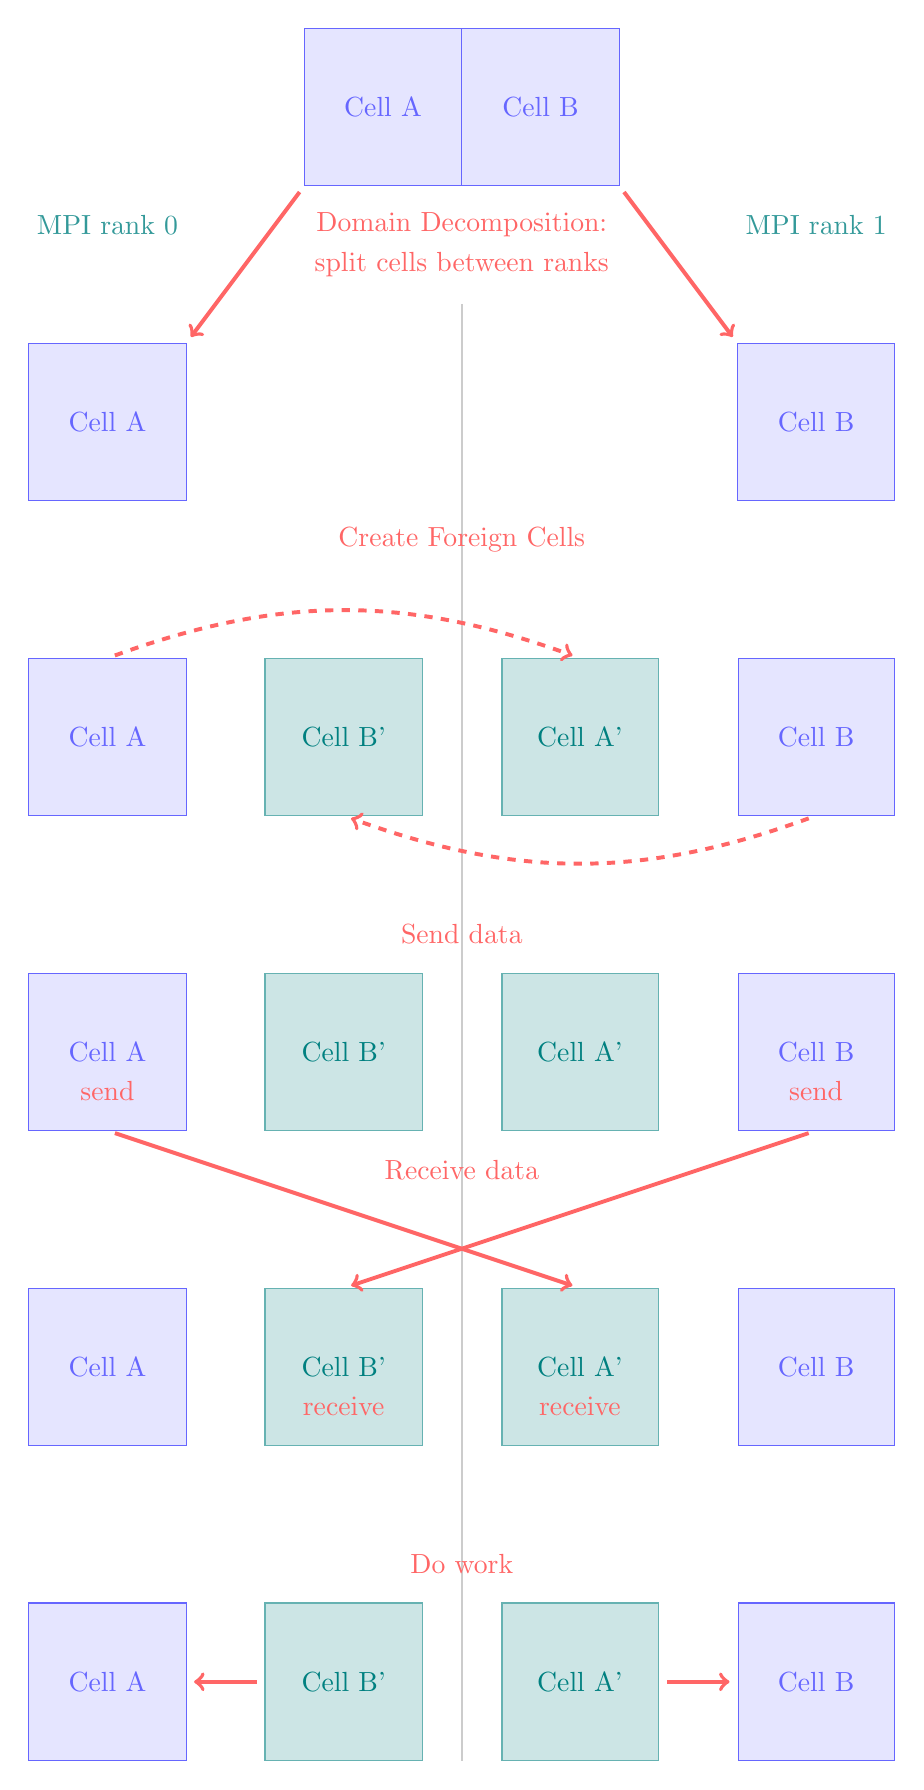
\begin{tikzpicture}[xscale=1,yscale=1,samples=400, transform shape,every node/.style={scale=1}]


\filldraw[fill=blue!10,draw=blue!60,line width=.15mm] (0.5,20) rectangle (2.5,22);
\filldraw[fill=blue!10,draw=blue!60,line width=.15mm] (2.5,20) rectangle (4.5,22);

\node[blue!60] (A1) at (1.5, 21) {Cell A};
\node[blue!60] (B1) at (3.5, 21) {Cell B};

\draw[line width=0.2mm, black!20] (2.5,18.5) -- (2.5,0);





\filldraw[fill=blue!10,draw=blue!60,line width=.15mm] (-3,20 - \ysep) rectangle (-1,22 - \ysep);
%\filldraw[fill=orange!20,draw=orange!60,line width=.15mm] (0, 20 - \ysep) rectangle (2, 22 - \ysep);
%\filldraw[fill=orange!20,draw=orange!60,line width=.15mm] (3.01, 20 - \ysep) rectangle (5., 22 - \ysep);
\filldraw[fill=blue!10,draw=blue!60,line width=.15mm] (6.0, 20 - \ysep) rectangle (8., 22 - \ysep);
\node[blue!60] (A2) at (-2, 21-\ysep) {Cell A};
\node[blue!60] (B2) at (7, 21-\ysep) {Cell B};


\draw[\instructioncolor, ->, line width=0.5mm, shorten >=0.1cm, shorten <=0.1cm] (0.5, 20) -- (-1, 22 - \ysep);
\draw[\instructioncolor, ->, line width=0.5mm, shorten >=0.1cm, shorten <=0.1cm] (4.5, 20) -- (6, 22 - \ysep);
\node[\instructioncolor] (domainDec) at (2.5, 19.5) {Domain Decomposition:};
\node[\instructioncolor] (domainDec2) at (2.5, 19.) {split cells between ranks};
\node[\rankcolor] (rank0) at (-2, 19.5) {MPI rank 0};
\node[\rankcolor] (rank1) at (7, 19.5) {MPI rank 1};


\filldraw[fill=blue!10,draw=blue!60,line width=.15mm] (-3,20 - 2*\ysep) rectangle (-1,22 - 2*\ysep);
\filldraw[fill=teal!20,draw=teal!60,line width=.15mm] (0, 20 - 2*\ysep) rectangle (2, 22 - 2*\ysep);
\filldraw[fill=teal!20,draw=teal!60,line width=.15mm] (3.01, 20 - 2*\ysep) rectangle (5., 22 - 2*\ysep);
\filldraw[fill=blue!10,draw=blue!60,line width=.15mm] (6.01, 20 - 2*\ysep) rectangle (8., 22 - 2*\ysep);
\node[blue!60] (A2) at (-2, 21-2*\ysep) {Cell A};
\node[blue!60] (B2) at (7, 21-2*\ysep) {Cell B};
\node[teal!100] (A2) at (1, 21-2*\ysep) {Cell B'};
\node[teal!100] (B2) at (4, 21-2*\ysep) {Cell A'};



\node[\instructioncolor] (foreign) at (2.5, 19.5-\ysep) {Create Foreign Cells};
\draw[->, \instructioncolor, line width=0.5mm, shorten >=0.1cm, shorten <=0.1cm, style=dashed] (-2, 21-2*\ysep+1) to[bend right=-20] (4, 21-2*\ysep+1);
\draw[->, \instructioncolor, line width=0.5mm, shorten >=0.1cm, shorten <=0.1cm, style=dashed]  (7, 21-2*\ysep-1) to[bend right=-20] (1, 21-2*\ysep-1) ;


\filldraw[fill=blue!10,draw=blue!60,line width=.15mm] (-3,20 - 3*\ysep) rectangle (-1,22 - 3*\ysep);
\filldraw[fill=teal!20,draw=teal!60,line width=.15mm] (0, 20 - 3*\ysep) rectangle (2, 22 - 3*\ysep);
\filldraw[fill=teal!20,draw=teal!60,line width=.15mm] (3.01, 20 - 3*\ysep) rectangle (5., 22 - 3*\ysep);
\filldraw[fill=blue!10,draw=blue!60,line width=.15mm] (6.01, 20 - 3*\ysep) rectangle (8., 22 - 3*\ysep);
\node[blue!60] (A2) at (-2, 21-3*\ysep) {Cell A};
\node[\instructioncolor] (A2) at (-2, 21-3*\ysep-0.5) {send};
\node[blue!60] (B2) at (7, 21-3*\ysep) {Cell B};
\node[\instructioncolor] (B2) at (7, 21-3*\ysep-0.5) {send};
\node[teal!100] (A2) at (1, 21-3*\ysep) {Cell B'};
\node[teal!100] (B2) at (4, 21-3*\ysep) {Cell A'};

\node[\instructioncolor] (foreign) at (2.5, 19.5-2*\ysep-1) {Send data};



\filldraw[fill=blue!10,draw=blue!60,line width=.15mm] (-3,20 - 4*\ysep) rectangle (-1,22 - 4*\ysep);
\filldraw[fill=teal!20,draw=teal!60,line width=.15mm] (0, 20 - 4*\ysep) rectangle (2, 22 - 4*\ysep);
\filldraw[fill=teal!20,draw=teal!60,line width=.15mm] (3.01, 20 - 4*\ysep) rectangle (5., 22 - 4*\ysep);
\filldraw[fill=blue!10,draw=blue!60,line width=.15mm] (6.01, 20 - 4*\ysep) rectangle (8., 22 - 4*\ysep);
\node[blue!60] (A2) at (-2, 21-4*\ysep) {Cell A};
\node[\instructioncolor] (A2) at (1, 21-4*\ysep-0.5) {receive};
\node[blue!60] (B2) at (7, 21-4*\ysep) {Cell B};
\node[\instructioncolor] (B2) at (4, 21-4*\ysep-0.5) {receive};
\node[teal!100] (A2) at (1, 21-4*\ysep) {Cell B'};
\node[teal!100] (B2) at (4, 21-4*\ysep) {Cell A'};

\node[\instructioncolor] (foreign) at (2.5, 19.5-3*\ysep) {Receive data};

\draw[->, \instructioncolor, line width=0.5mm, shorten >=0.1cm, shorten <=0.1cm] (-2, 21-3*\ysep-1) to (4, 21-4*\ysep+1);
\draw[->, \instructioncolor, line width=0.5mm, shorten >=0.1cm, shorten <=0.1cm]  (7, 21-3*\ysep-1) to (1, 21-4*\ysep+1) ;



\filldraw[fill=blue!10,draw=blue!60,line width=.15mm] (-3,20 - 5*\ysep) rectangle (-1,22 - 5*\ysep);
\filldraw[fill=teal!20,draw=teal!60,line width=.15mm] (0, 20 - 5*\ysep) rectangle (2, 22 - 5*\ysep);
\filldraw[fill=teal!20,draw=teal!60,line width=.15mm] (3.01, 20 - 5*\ysep) rectangle (5., 22 - 5*\ysep);
\filldraw[fill=blue!10,draw=blue!60,line width=.15mm] (6.01, 20 - 5*\ysep) rectangle (8., 22 - 5*\ysep);
\node[blue!60] (A2) at (-2, 21-5*\ysep) {Cell A};
\node[blue!60] (B2) at (7, 21-5*\ysep) {Cell B};
\node[teal!100] (A2) at (1, 21-5*\ysep) {Cell B'};
\node[teal!100] (B2) at (4, 21-5*\ysep) {Cell A'};

\node[\instructioncolor] (foreign) at (2.5, 18.5-4*\ysep) {Do work};

\draw[<-, \instructioncolor, line width=0.5mm, shorten >=0.1cm, shorten <=0.1cm] (-1, 21-5*\ysep) -- (0, 21-5*\ysep);
\draw[<-, \instructioncolor, line width=0.5mm, shorten >=0.1cm, shorten <=0.1cm] (6, 21-5*\ysep) -- (5, 21-5*\ysep);




	\end{tikzpicture}
\end{document}